\title{Functional Magnetic Resonance Imaging and Blood Oxygen Level Dependent Signal}
\label{cha:intro}

\section{Functional Imaging of the Human Brain}

For over a century, neuroscientists and neurophysiologists have dedicated their
efforts to uncovering the functional organization of the brain. Through the use
of various functional neuroimaging techniques with complementary temporal and
spatial resolutions, they aim to reveal the neuro-anatomical localization and
dynamic changes of brain activations.

While non-invasive electrophysiological techniques such as
electroencephalography (EEG) or magnetoencephalography (MEG) excel in temporal
resolution (10-100 ms), their spatial resolution is relatively poor (several mm
or cm)
\citep{Baillet2001Electromagneticbrainmapping,Haemaelaeinen1993Magnetoencephalographytheoryinstrumentationapplications}.
In contrast, invasive electrophysiological techniques, including patch clamps
\citep{Neher1978extracellularpatchclamp}, single-unit or multi-unit recordings
\citep{Arieli1995Coherentspatiotemporalpatterns}, and electrocorticography
(\acrshort*{ecog})
\citep{Miller2007Realtimefunctional,Nir2008Interhemisphericcorrelationsslow},
offer high spatial resolution.

Functional magnetic resonance imaging (fMRI) and Positron Emission Tomography
(PET) provide insight into cerebral blood flow and oxygen metabolism, indirectly
associated with neural activations. With spatial resolutions in the order of
millimeters, these techniques are capable of capturing activations in both
cortical and deep brain structures, but their temporal resolution is limited by
the sluggish dynamics of hemodynamic changes
\citep{Dale2001Spatiotemporalmappingbrain}. fMRI offers higher temporal and
spatial resolution compared to \acrshort*{pet}, making it more suitable for
studying the temporal responses to short neuronal-related events. However, PET
has the advantage of measuring well-defined physiological quantities such as
cerebral blood flow (CBF), cerebral blood volume (CBV), or cerebral metabolic
rate of oxygen or \acrshort*{cmro2}
\citep{Fox1986Mappinghumanvisual,Friston1993FunctionalConnectivityPrincipal}.

Functional MR spectroscopy (MRS) is an alternative method for metabolic imaging,
offering quantitative measurements of functional changes in neurometabolite and
neurotransmitter concentrations within a specific brain region. However, it is
important to note that MRS has lower spatial and temporal resolutions compared
to fMRI \citep{Morris1999Magneticresonanceimaging}. Typically, MRS is performed
in a single voxel with an isotropic size of a few centimeters, or in multiple
voxels using chemical shift imaging.

Lastly, optical diffusion imaging techniques, such as near infrared spectroscopy
(NIRS)
\citep{Kleinschmidt1996SimultaneousRecordingCerebral,Villringer1993infraredspectroscopyNIRS},
diffusion optical tomography (DOT) \citep{White2010Quantitativeevaluationhigh},
or event-related optical signaling (EROS)
\citep{Gratton2001eventrelatedoptical,Gratton1997FastLocalizedEvent}, utilize an
optical imaging device placed on the scalp to measure changes in cortical blood
flow. However, due to the need for the light to penetrate through the skull,
these techniques have lower spatial resolution compared to MR imaging techniques
and are limited to studying the cortical surface. The temporal resolution of
\acrshort*{eros} is similar to \acrshort*{meg} and \acrshort*{eeg} (in the order
of milliseconds), while \acrshort*{nirs} has a ten times higher temporal
resolution to fMRI.A notable advantage of optical imaging is its lower cost and
portability compared to other techniques such as MRI or MEG.

\section{Blood Oxygen Level Dependent Functional MRI}

In order to fully comprehend the assumptions and methods presented in this
thesis, it is essential to review some basic concepts related to the physical
and physiological basis of the blood oxygen-level dependent (BOLD) effect. MRI
techniques offer a range of approaches to detect the increased metabolic demand
associated with brain function. These include utilizing the BOLD contrast,
changes in \acrshort*{cbv} using contrast agents such as gadolinium
\citep{Dean1992CerebralHA}, ferumoxytol
\citep{Christen2012Highresolutioncerebral} or hyperoxic contrasts
\citep{Bulte2007Measurementcerebralblood}, and assessing \acrshort*{cbf} through
arterial spin labeling techniques (\acrshort*{asl})
\citep{Buxton2009IntroductionFunctionalMagnetic}. BOLD fMRI, introduced by
\cite{Ogawa1990Brainmagneticresonance,Ogawa1992Intrinsicsignalchanges}, is
particularly advantageous as it requires no exogenous contrast agent and
exhibits higher sensitivity compared to CBF-based contrast, such as ASL.
Consequently, it has gained widespread usage for functional brain imaging.

\subsection{Physiological Basis of the BOLD Constrast}

The signal contrast in BOLD fMRI images arises from variations in the local
magnetic susceptibility, $\chi$, caused by disparities in blood hemoglobin
oxygen concentration. As local neuronal activity intensifies, there is a rise in
oxygen consumption, leading to an augmented supply of oxygenated blood that
diffuses passively through the capillary blood vessels to the tissue. When
oxygen binds to hemoglobin (forming oxyhemoglobin), it exhibits slight
diamagnetic properties relative to the tissue, causing the molecule to repel the
magnetic field. In contrast, deoxygenated hemoglobin is paramagnetic compared to
the tissue, attracting the magnetic field. Consequently, the magnetic field
becomes distorted near deoxygenated red blood cells, creating higher local
magnetic field gradients in the surrounding tissue, which results in spin
dephasing. Reduced oxygenation amplifies the spin dephasing effect, shortening
the tissue's $T_2^*$ and diminishing the amplitude of the MR signal in
$T_2^*$-weighted images. Conversely, higher oxygen concentration aligns the
susceptibility of the blood with that of the surrounding tissue, reducing the
local magnetic field gradient, increasing $T_2^*$, and raising the measured MR
signal amplitude by a few percent. This forms the basis of BOLD fMRI, where
changes in blood oxygenation serve as an intrinsic contrast mechanism in
$T_2^*$-weighted images, enabling the identification of cortical regions
exhibiting functional activity characterized by increased oxygen demand and
supply
\citep{Bandettini1992TimecourseEPI,Belliveau1991FunctionalMappingHuman,Kwong1992Dynamicmagneticresonance,Ogawa1990Brainmagneticresonance,Ogawa1992Intrinsicsignalchanges,Turner1991Echoplanartime}.

\subsection{Temporal Characteristics of the BOLD Signal: the Hemodynamic Response Function}

The BOLD effect does not directly reflect neuronal activity, but rather measures
the hemodynamic response associated with it
\citep{Logothetis2008Whatwecan,Logothetis2001Neurophysiologicalinvestigationbasis}.
The relationship between the hemodynamic response and the underlying neuronal
activity is complex involving dynamic changes in CBF, CBV and $CMRO_2$
\citep{Buxton2009IntroductionFunctionalMagnetic}. After neuronal activity
increases in a brain region, there is an initial decrease in blood oxygenation
due to oxygen consumption which might cause a small initial dip in the
hemodynamic response following the first second after the activation
\citep{Ernst1994Observationfastresponse,Menon1995BOLDBasedFunctional}. Although
this initial dip is not always observed in fMRI
\citep{Behzadi2006Caffeinereducesinitial,Buxton2009IntroductionFunctionalMagnetic,Hu1997Evaluationearlyresponse,Hu1997Evaluationearlyresponse},
it is suggested that it maps more accurately the site of neural activity
\citep{Duong2000SpatiotemporaldynamicsBOLD,Malonek1996InteractionsElectricalActivity}.
Afterwards, the local supply of oxyhemoglobin increases more than it is strictly
demanded, probably to ensure a large oxygen gradient across capillary walls so
that there is a high rate of transfer of oxygen or glucose to tissue
\citep{Logothetis2008Whatwecan}, generating a positive BOLD response due to an
excess of oxyhemoglobin. Negative BOLD responses have also been observed
associated with neuronal deactivations \citep{Shmuel2006NegativefunctionalMRI}.
Regardless of the polarity of the response, the BOLD response peaks between 5
and 8 s after the activation starts and its amplitude depends on the type of
stimulus and the magnetic field strength. For instance, for visual stimulation
the signal change is 2-3 \% at 1.5T, 4-6 \% at 3T, 7-10 \% at 7T
\citep{Zwaag2009fMRI1.53}. After the stimulus ceases, there is a return of the
BOLD response to baseline, often followed by a post-stimulus undershoot due to
an increase of deoxyhemoglobin which may last for several seconds until the
response returns to baseline. The cause of the post-stimulus undershoot is also
not completely understood, whether this is a vascular, neural or metabolic
effect \citep{Buxton2009IntroductionFunctionalMagnetic,Chen2009OriginsBOLDpost}.
In summary, the time scale of the BOLD response is much slower than the time
scale of neural activity and the return of the BOLD signal to baseline level
after a short stimulus may occur more than 30 s from the stimulus onset. The
temporal characteristics of the BOLD response are usually modelled by a
hemodynamic response function (HRF). \cref{fig:hrf_shape} shows the shape of
typical HRF, along with the initial dip for illustration of this effect. In this
figure, the HRF plotted is the well-known canonical HRF
\citep{Friston2007Statisticalparametricmapping,Friston1998EventRelatedfMRI},
which is defined as the difference of two-gamma functions:
\begin{figure}[t!]
    \centerline{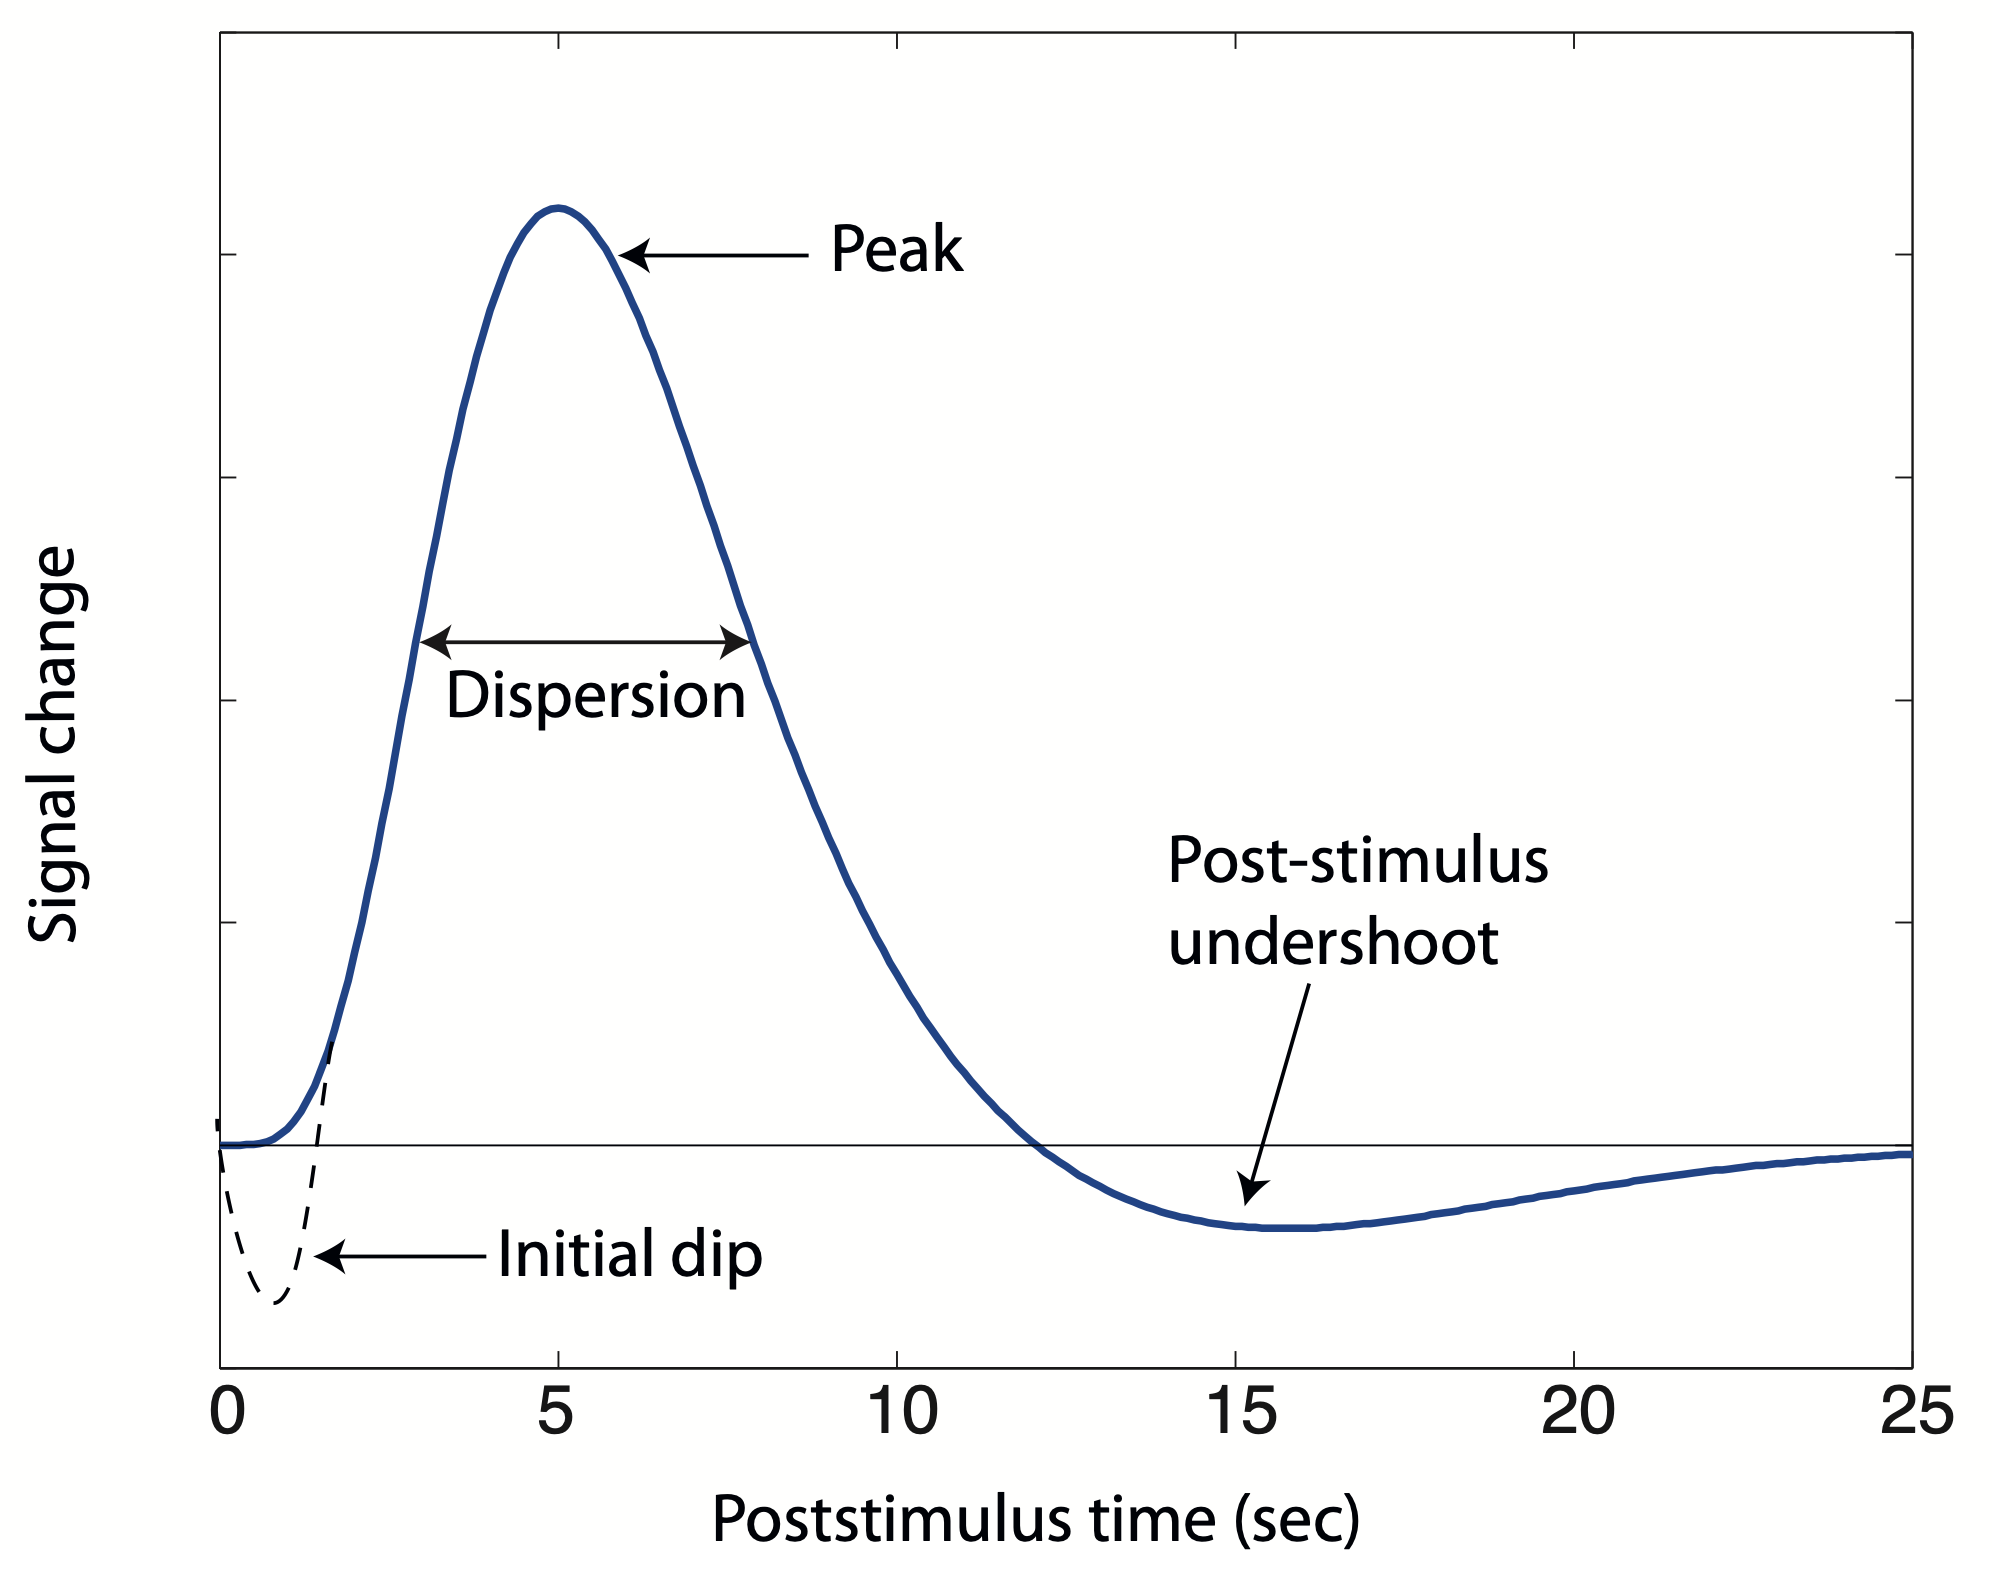
\includegraphics[width=\textwidth]{figures/introduction/hrf_shape.png}}
    \caption{Temporal characterization of the haemodynamic response function.
    The shape in bold line corresponds to the canonical haemodynamic response
    function.}
\label{fig:hrf_shape}
\end{figure}

\begin{equation}
    h(t)=g(t; a_1, b_1) - \frac{1}{c}g(t; a_2, b_2),
\end{equation}
where the Gamma function is given by

\begin{equation}
    g(t; a, b) = \frac{b^a t^{a-1} e^{-bt}}{\Gamma(a)}.
\end{equation}

The canonical HRF, as described in literature
\citep{Friston2007Statisticalparametricmapping}, is characterized by specific
parameters. These parameters include a time-to-peak $(a/b)$ of 6 s and
dispersion $(a/b^2)$ of 1 s for the initial overshoot. Additionally, it has a
time-to-peak of 16 s and dispersion of 1 s for the undershoot. The
overshoot-undershoot ratio $(c)$ is approximately 6. However, it is important to
note that the BOLD response exhibits variability across trials, brain regions,
and subjects
\citep{Aguirre1998VariabilityHumanBOLD,Duann2002SingleTrialVariability,Handwerker2004VariationBOLDhemodynamic,McGonigle2000VariabilityfMRIExamination,Smith2005VariabilityfMRIre}.
To account for this variability, alternative HRF shapes have been proposed in
the scientific literature. These include single gamma functions
\citep{Boynton1996LinearSystemsAnalysis,Cohen1997ParametricAnalysisfMRI},
two-gamma functions with different HRF parameters
\citep{Glover1999DeconvolutionImpulseResponse}, Poisson functions
\citep{Friston1994AnalysisfunctionalMRI}. and Gaussian functions
\citep{Kruggel1999Modelinghemodynamicresponse,Rajapakse1998Modelinghemodynamicresponse}.

\section{Noise in BOLD fMRI}

In addition to neuronal-related activity, the BOLD signal presents multiple
sources of noise related to hardware-related artifacts and drifts, head motion,
confounding physiological fluctuations
\citep{Bianciardi2009Sourcesfunctionalmagnetic,Jorge2013SignalfluctuationsfMRI}
as well as image distortions related to data acquisition that should be
accounted for and corrected during fMRI data preprocessing.

\subsection{Motion and Other Artifacts}

For instance, the images could present geometric distortions in the phase
direction of the acquisition that can be removed by means of mapping field
distorsions, either using field maps or using two images acquired in opposite
phase-encoding directions, and then with a non-linear transformation of the fMRI
volumes (e.g. TOPUP,
\cite{Andersson2003Howcorrectsusceptibility,Glasser2018UsingtemporalICA}). Also,
fMRI images are typically acquired slice by slice and the difference in their
time of acquisition can be compensated via slice timing correction, although
this step can also introduce confounding effects in the data due to signal
interpolation \citep{Parker2019BenefitSliceTiming}. More generally, realigning
all fMRI volume to a reference image can deal with part of the artifacts
introduced by head motion \citep{Friston1994Statisticalparametricmaps}. However,
this step does not remove the effect of motion completely
\citep{CaballeroGaudes2017MethodscleaningBOLD}.

The most straight-forward way to deal with signal artifacts is to model them as
regressors of non-interest along with the task regressors (in tIA-fMRI) or to
project them out of the fMRI data if there is no task paradigm, as in
resting-state (RS) experiments. For instance, motion-related effects can be
expressed as a set of the relative translations and rotation obtained during
realignment, considering their first derivative and their squared transformation
for up to 24 regressors for a better denoising
\citep{Friston1994Statisticalparametricmaps}. Similarly, very low frequency
trends due to hardware-related inestabilities can be modelled as a set of basis
functions (e.g. using Legendre polynomials, Discrete Cosine Transform).

Furthermore, large deviations in the fMRI signal (e.g., spikes) caused by motion
jerks and scanner noise can be removed through scrubbing or censoring
\citep{Power2012Spurioussystematiccorrelations}. This process consists in
identifying those fMRI volumes characterized by abrupt changes in the BOLD
signal and removing or interpolating them. The identification can be performed
by using summary metrics of motion, like Framewise Displacement
\citep{Power2012Spurioussystematiccorrelations}, or by observing transient
changes in the signal (DVARS, \cite{Power2012Spurioussystematiccorrelations,
Smyser2010LongitudinalAnalysisNeural}). However, it is important to notice that,
if correctly accounted for, scrubbing could reduce the degrees of freedom in
statistical analysis \citep{Mascali2021Evaluationdenoisingstrategies}, leading
to biases in second-level analysis between subjects that move too much and
others, or introduce discontinuity in the signal itself, limiting the use of
particular analyses dependent on signal continuity (e.g. \acrshort*{ica}, see
\cite{CaballeroGaudes2017MethodscleaningBOLD}), and biasing the estimation of
functional connectivity \citep{Mascali2021Evaluationdenoisingstrategies}.
Moreover, interpolating the signal could introduce spurious changes in the
signal.

Another common approach to remove not only motion, but also other sources of
noise, is based on data decomposition techniques. For instance, ICA can be
leveraged to model, identify and remove motion artifacts as well as other
sources of noise
\citep{Behzadi2007componentbasednoise,Griffanti2014ICAbasedartifact,Muschelli2014Reductionmotionrelated,Pruim2015ICAAROMArobust,Pruim2015EvaluationICAAROMA,SalimiKhorshidi2014Automaticdenoisingfunctional}.
Ideally, the best candidate to identify noisy timeseries would be temporal ICA,
i.e., a decomposition in which the independence is forced in the temporal domain
\citep{Glasser2018UsingtemporalICA,Smith2012Temporallyindependentfunctional}.
However, such approach is not feasible in a normal fMRI context since it would
require the samples in time to be much higher than the samples in space
\citep{Smith2012Temporallyindependentfunctional}. Hence, spatial ICA is the most
common application for fMRI decomposition, although this might lead to detect
spurious components that contain both true BOLD signal and noise
\citep{CaballeroGaudes2017MethodscleaningBOLD}. Alternatively, several fMRI
sessions could be concatenated to apply temporal ICA, although this approach
would lead to the impossibility of removing session-specific noise. The
challenging factor in adopting ICA for denoising is the classification of the
independent components. Although manual classification is still the approach
with the best outcome \citep{Griffanti2017HandclassificationfMRI}, it is time
consuming, it requires trained researchers, and the result is dependent on the
observer. For this reason, different approaches for automatic classification of
ICA components have been proposed in time, from full classifiers (FIX,
\cite{SalimiKhorshidi2014Automaticdenoisingfunctional}) to approaches
specifically targeting motion artifacts (ICA-AROMA,
\cite{Pruim2015ICAAROMArobust,Pruim2015EvaluationICAAROMA}).

Alternatively, decomposing the signal of white matter (\acrshort*{wm}) and
cerebrospinal fluid (\acrshort*{csf}) into principal components and considering
the first few (a technique called anatomical CompCor, see
\cite{Behzadi2007componentbasednoise}) can help retrieving proxies of
motion-related artifacts and physiological fluctuations
\citep{Behzadi2007componentbasednoise,Muschelli2014Reductionmotionrelated}. In
fact, it has been shown that CompCor can be more effective in denoising motion
artifacts than ICA based techniques and censoring
\citep{Mascali2021Evaluationdenoisingstrategies}.

Noise in fMRI can also be reduced by using multi-echo (ME) acquisitions that
sample the data at multiple successive echo times (\acrshort*{te}). A weighted
combination of the multiple echoes based on each voxel's $T_2^*$ value
\citep{Posse1999EnhancementBOLDcontrast} or temporal signal-to-noise ratio
\citep{Poser2006BOLDcontrastsensitivity} can smear out random noise and enhance
the sensitivity to the BOLD contrast. In fact, compared with single-echo data,
this optimal combination \citep{Liu2022geometricviewsignal} can improve the
mapping of neuronal activity at 3T \citep{Fernandez2017MultiechoEPI} and 7T
\citep{Puckett2018Usingmultiecho}, with results comparable to other
preprocessing techniques requiring extra data such as RETROICOR
\citep{Atwi2018AttentionRelatedBrain}. Optimal combination of multiple echo
volumes can also improve sensitivity, specificity, repeatability and reliability
of fMRI mapping
\citep{Cohen2021ImprovingBreathHolding,Cohen2019ImprovingAssessmentBreath}.

Furthermore, assuming a monoexponential decay, the voxelwise fMRI signal
acquired at a given echo time TE, i.e. $S(TE)$, can be expressed in signal
percentage change as:
\begin{equation}
    \frac{S(TE)-\overline{S}(TE)}{\overline{S}(TE)}\approx \Delta \rho - \text{TE} \cdot \Delta R_2^* + n,
\end{equation}
where $\overline{S}(TE)$ is the average signal at a given TE, $\Delta \rho$
represents non-BOLD related changes in the net magnetisation, $\Delta R_2^*$
represents BOLD-related susceptibility changes (and is the inverse of $\Delta
T_2^*$), and $n$ denotes random noise
\citep{Kundu2013Integratedstrategyimproving,Kundu2012DifferentiatingBOLDnon}. As
the BOLD-related signal can be expressed as a function of the TE, whereas
noise-related (i.e., non-BOLD) changes in the net magnetization are independent
of TE, the information available in multiple echoes can be leveraged for the
purpose of denoising. For example, in a dual-echo acquisition where the first TE
is suficiently short, the first echo signal mainly captures changes in $\Delta
\rho$ rather than in $\Delta R_2^*$. It is then possible to remove artifactual
effects, through voxelwise regression, from the second echo signal acquired at a
longer TE with appropriate BOLD contrast
\citep{Bright2013Removingmotionphysiological}.

Collecting more echoes opens up the possibility to leverage ICA and
automatically classifying independent components into BOLD-related (i.e.,
describing $\Delta R_2^*$ fluctuations with a linear TE-dependency) or noise
(i.e., independent of TE, related to non-BOLD fluctuations in the net
magnetization $\Delta \rho$), an approach known as \acrshort*{me} independent
component analysis (ME-ICA,
\cite{Kundu2013Integratedstrategyimproving,Kundu2012DifferentiatingBOLDnon,Kundu2017MultiechofMRI}).
Compared to single-echo data denoising, \acrshort*{meica} can improve the
mapping of task-induced activation
\citep{DuPre2021TEdependentanalysis,GonzalezCastillo2016Evaluationmultiecho,Lombardo2016Improvingeffectsize},
for example in challenging paradigms with slow-varying stimuli
\citep{Evans2015SeparatingslowBOLD} or language mapping and laterality
\citep{Amemiya2018Integratedmultiecho}. It also outperforms single-echo
ICA-based denoising of resting-state fMRI data
\citep{Dipasquale2017Comparingrestingstate,Lynch2020RapidPrecisionFunctional},
and provide more effcient and reliable functional connectivity mapping in
individual subjects \citep{Lynch2020RapidPrecisionFunctional} and in brain
regions where traditional single-echo acquisitions offer reduced signal-to-noise
ratio, such as the basal forebrain \citep{Markello2018Segregationhumanbasal}.
Finally, ME-ICA also enhances the deconvolution of neuronal-related signal
changes \citep{CaballeroGaudes2019deconvolutionalgorithmmulti}.

\subsection{Physiological Artifacts}

When employing BOLD fMRI as an intrinsic contrast to investigate neural
correlates, it becomes essential to decouple the neurovascular coupling. In this
context, physiological signals may introduce noise, requiring their modeling to
account for and minimize their associated variance during preprocessing or data
analyses \citep{CaballeroGaudes2017MethodscleaningBOLD,
Liu2016NoisecontributionsfMRI}. The principal frequencies characterising
physiological signals like cardiac pulse and respiration are in a different band
compared to those of the neural-related BOLD signal: namely, the primary
component of cardiac related fluctuations are around 1 Hz, while the respiratory
related ones are around 0.3 Hz. Thus, if the temporal sampling is high enough, a
simple band-pass filter could easily remove their confounding effects
\citep{Biswal1995Functionalconnectivitymotor,Chuang2001IMPACTImagebased,Lowe1998FunctionalConnectivitySingle}.
The downside is that this approach will remove the BOLD-related signal
frequencies in the same range as well, and it will not remove the impact of
physiological frequencies in the same range as the BOLD signal
\citep{CaballeroGaudes2017MethodscleaningBOLD}. This is especially true if the
temporal sampling is low and the physiological signal is aliased in the
BOLD-related frequency range. Moreover, physiological signal, and respiration in
particular, has an impact on other sources of noise, like magnetic field
perturbation \citep{Raj2001Respiratoryeffectshuman}, and motion
\citep{Fair2020Correctionrespiratoryartifacts,PaisRoldan2018IdentifyingRespirationRelated,Power2019Distinctionsrealapparent}
that should be taken into account and removed
\citep{Gratton2020Removalhighfrequency}.

An easy way to remove such perturbations is to remove the average brain signal
(also called global signal), since it is often considered as a proxy of the
combined impact of different sources of noise, especially related to movement or
physiological in nature. However, its removal is controversial, since it can
heavily alter the interpretation of BOLD fMRI
\citep{Power2017Sourcesimplicationswhole}. For this reason,
\cite{Power2018RiddingfMRIdata} proposed to decompose fMRI data in low and high
rank components, and to consider the first few low rank components timeseries as
noise. This technique, called GODEC, showed improved denoising of fMRI data
after ME-ICA \citep{Power2018RiddingfMRIdata,Zhou2011GoDecRandomizedlow}.

As an alternative, the average signal in the white matter (WM) and cerebrospinal
fluid (CSF) can be used as a proxy of physiological noise, since no
neural-related signal is present in these tissues, that are conversely dominated
by cardiac pulsatility and respiration
\citep{Anderson2011Networkanticorrelationsglobal,Jo2010Mappingsourcescorrelation},
although more recently \cite{Attarpour2021Vascularoriginslow} showed that the
average CSF does not represent cardiac fluctuations properly. Specifically, ICA
based decomposition can be set up to retrieve physiological-related signals,
both in space (CORSICA, \cite{Perlbarg2007CORSICAcorrectionstructured}) and in
time (PESTICA, \cite{Beall2007Isolatingphysiologicnoise}).

An alternative to data-driven approaches consists in acquiring physiological
signals such as cardiac pulse and respiration effort during the imaging session,
opening up the possibility to adopt more model-based approaches to deal with
physiological noise. For instance, it is possible to estimate the frequencies of
the amplitude envelope of cardiac and respiratory signals, and then selectively
filter them from fMRI data \citep{Biswal1996Reductionphysiologicalfluctuations}.
However, the main frequency and the harmonics of physiological fluctuations are
usually aliased with the spectra of BOLD components with neurobiological
relevance, and bandpass filtering would remove them as well.

Alternatively, it is possible to use the measured cardiac and respiratory
signals to model their pseudo-periodic fluctuation that are phase-locked to the
fMRI signal. Cardiac and respiratory phases can be estimated from signal
recordings, then their Fourier expansion can be removed from the data in a
slice-dependent manner at the beginning of the preprocessing, an approach known
as RETROICOR, \cite{Glover2000Imagebasedmethod}. However, RETROICOR does not
remove completely the effect of physiological signal from the data, especially
regional low frequency effects that vary between brain regions
\citep{Birn2006Separatingrespiratoryvariation,Chang2009Influenceheartrate,Shmueli2007Lowfrequencyfluctuations}.

Noticeably, slow variations in the heart rate (HR,
\cite{Shmueli2007Lowfrequencyfluctuations}) and the respiration volume per time
(RVT, \cite{Birn2006Separatingrespiratoryvariation}) have been applied
successfully to denoise BOLD signal from physiological fluctuations after
RETROICOR, especially when convolved with a modelled response function, cardiac
\citep{Chang2009Influenceheartrate} or respiratory
\citep{Birn2008respirationresponsefunction}. Various alternatives to
\acrshort*{rvt} to improve breathing-related denoising have been proposed,
either to simplify their calculation, that is normally based on the peak
detection in the respiratory signal, or to improve the detection of particular
changes in the respiratory signal. For instance,
\cite{Chang2009Relationshiprespirationend} proposed to simply use the standard
deviation of the respiratory signal, thus avoiding peak detection.
\cite{Power2018RiddingfMRIdata} suggested to compute the standard deviation of
the respiratory envelope in small windows to be more susceptible to breathing
changes\cite{I think this is not the proper reference by Power for this method}.
More recently, \cite{Harrison2021Hilbertbasedmethod} showed that applying an
Hilbert transform to compute RVT improves the characterisations of breathing
rhythms and the detection of deep breaths. Although the regions impacted by slow
variations in cardiac rate and breathing patterns frequently overlap
\citep{Chang2009Influenceheartrate,Kassinopoulos2019Identificationphysiologicalresponse},
\acrshort*{hr} and RVT regressor can be used together for better performance
\citep{Chang2009Influenceheartrate}.

Another physiological confound related to RVT consists in spontaneous changes in
arterial CO2, called poikilocapnia, which act as a vasoactive process. These
fluctuations have been corroborated with Transcranial Doppler ultrasound
(\acrshort*{tcd}) and induce low frequency fluctuations in the BOLD signal. If
they are not accounted for, they can induce a bias in the signal estimation in
up to a fifth of the cortex \citep{Wise2004Restingfluctuationsarterial}. The
pattern of biases induced by poikilocapnia has been found comparable to that of
RVT \citep{Chang2009Relationshiprespirationend}, although accounting for the
latter is not suffcient to explain all the variability induced by the former
\citep{Golestani2015Mappingendtidal}. However, the fact that BOLD signal is
susceptible to CO2 fluctuations can be conversely seen as an advantage, and used
to image cerebral physiology
\citep{Pinto2021CerebrovascularReactivityMapping,Zvolanek2023Comparingendtidal,Moia2021ICAbaseddenoising}.

\section{fMRI Data Analysis}

\subsection{Task fMRI}

Conventionally, the analysis of task fMRI data consists of solving a generalized
liner model (GLM) analysis. Since researchers have access to the timings of the
stimuli, it is possible to model the expected BOLD response to the stimuli and
then fit the model to the data. For instance, the onsets of the expected
neuronal activity for a given condition can be modeled as an indicator function
$p(t)$ (e.g., Dirac functions for event-related designs, or box-car functions
for block-designs) convolved with the HRF $h(t)$, sampled at the resolution of
the TR
\citep{Friston2008DEMvariationaltreatment,Friston1998EventRelatedfMRI,Boynton1996LinearSystemsAnalysis,Cohen1997ParametricAnalysisfMRI}:
\begin{equation}
    x(t) = p \times h(t) \rightarrow x\left[k\right] = p \times h(k \cdot \text{TR}).
\end{equation}

Hence, the vector $\mathbf{x} = \left[x\left[k\right]\right]_{k=1,\dots,N} \in
\mathbb{R}^N $ represents the regressor that models the hypothetical BOLD
response for an experimental condition. Then, different regressors either
modeling conditions of interest or signals of non interest (e.g., noise-related
signals) can be added as the columns of the design matrix $\mathbf{X} =
\left[\mathbf{x}_1, \dots, \mathbf{x}_L\right] \in \mathbb{R}^{N\times L}$,
where $L$ is the number of regressors, which leads to the well-known
\acrshort*{glm} equation:
\begin{equation}
    \mathbf{y} = \mathbf{X} \mathbf{\beta} + \mathbf{\epsilon},
\end{equation}
where the voxel timecourse $\mathbf{y} \in \mathbb{R}^N$ is explained by a
linear combination of the regressors in $\mathbf{X}$, weighted by the regression
coefficients $\mathbf{\beta} \in \mathbb{R}^L$, and the residual error or noise
$\mathbf{\epsilon} \in \mathbb{R}^N$. The GLM can be solved using ordinary least
squares (OLS) under the assumption that the noise is independent and identically
distributed (i.i.d.) Gaussian. Hence, the estimates of neuronal activity
corresponding to the task conditions are obtained minimizing the residual sum of
squares between the fitted model and the measured voxel timecourse. Usually, the
number of regressors is much smaller than the number of samples, and thus the
GLM is an overdetermined problem. In this case, the solution can be obtained
without the need for additional constraints or assumptions
\citep{Henson2007CHAPTER14Convolution}. It is important to note that the GLM
only provides estimates of the neuronal activity associated with the timings of
the modelled stimuli.

\subsection{Resting-State fMRI}

Conversely, fMRI data analysis in unconstrained conditions such as when subjects
lying still in the scanner without performing any specific task, i.e. in
resting-state, poses a challenge for the application of GLM-based approaches due
to the absence of an experimental paradigm that can be used to model the
expected BOLD response. Given the increasing popularity of resting-state fMRI in
the past decade, various data-driven approaches have emerged to address the
analysis of this type of data. 

Seed correlation analysis is widely recognized as the predominant approach for
examining resting-state fMRI data due to its frequent utilization in the
computation of functional connectivity (FC) patterns. It involves measuring the
pairwise Pearson correlation between the timecourse of different voxels or
regions of the brain, presenting the brain's interregional connections or edges
in the form of a FC matrix. Each edge in the matrix represents the strength or
intensity of the functional connectivity between two regions. In fact,
\acrshort*{fc} has been extensively utilized to investigate the arrangement of
large-scale brain networks
\citep{Salvador2005NeurophysiologicalArchitectureFunctional,Yeo2011organizationhumancerebral,Margulies2016Situatingdefaultmode},
as well as to partition smaller brain structures like the thalamus and striatum
\citep{Martino2008FunctionalConnectivityHuman,Yuan2015Functionaltopographythalamocortical,Tian2020Topographicorganizationhuman}.
Notably, FC exhibits subject-specific variations to such an extent that it can
serve as a means of individual identification within a diverse population.
Numerous studies have demonstrated the presence of distinct and reliable
subject-specific features, commonly referred to as "fingerprints," within the FC
matrix \citep{MirandaDominguez2014ConnectotypingModelBased,
Finn2015Functionalconnectomefingerprinting, Finn2017Canbrainstate,
Vanderwal2017Individualdifferencesfunctional,
Waller2017Evaluatingreplicabilityspecificity,
Amico2018questidentifiabilityhuman, PenaGomez2017SpatiotemporalNetworkMarkers,
Horien2019individualfunctionalconnectome,
Jalbrzikowski2020Functionalconnectomefingerprinting,
Jo2021Subjectidentificationusing}. In fact, these fingerprints have been
associated with predictive insights into cognition
\citep{Cole2012GlobalConnectivityPrefrontal,Rosenberg2015neuromarkersustainedattention,Yamashita2018predictionmodelworking,Fong2019Dynamicfunctionalconnectivity,Rosenberg2020Functionalconnectivitypredicts,Sripada2019Predictionneurocognitionyouth},
personality traits
\citep{Adelstein2011PersonalityIsReflected,Hsu2018Restingstatefunctional,Nostro2018Predictingpersonalitynetwork,Dubois2018RestingStateFunctional},
age
\citep{Dosenbach2010PredictionIndividualBrain,Cabral2017Cognitiveperformancehealthy,Liem2017Predictingbrainage,Nielsen2018EvaluatingPredictionBrain},
and disease phenotype
\citep{Lynall2010FunctionalConnectivityBrain,Plitt2015Restingstatefunctional,Emerson2017Functionalneuroimaginghigh,Lake2019FunctionalBrainOrganization,Svaldi2021Optimizingdifferentialidentifiability}.

Functional connectivity patterns offer a valuable insight into the connectivity
among brain regions over a timecourse of data. However, they only provide a
single snapshot and do not capture how this connectivity evolves over time,
thereby neglecting the dynamics of functional connectivity.
\citep{Allen2012TrackingWholeBrain,Di2020Intersubjectconsistentdynamic,Hutchison2013Dynamicfunctionalconnectivity}.
Dynamic functional connectivity (dFC) in resting-state is commonly investigated
using sliding-window approaches
\citep{Allen2012TrackingWholeBrain,Hutchison2013Dynamicfunctionalconnectivity,Preti2017dynamicfunctionalconnectome,Lurie2020Questionscontroversiesstudy}.
A sliding-window FC analysis yields a series of time-varying matrices, which are
often effectively condensed into a few distinct brain states using clustering
techniques \citep{Hutchison2013Dynamicfunctionalconnectivity}. In particular, it
has been shown that \acrshort*{dfc} correlates with underlying neural activity
\citep{Tagliazucchi2012Criticalitylargescale,Thompson2013Neuralcorrelatestime,Keilholz2014NeuralBasisTime}
and behavior \citep{Liegeois2019Restingbraindynamics}. Furthermore, studies have
demonstrated that dynamic connectivity fluctuations exhibit lower variability
between regions within the same functional networks, while showing higher
variability between regions from different networks
\citep{Fu2017AssociationsFunctionalConnectivity}. This pattern results in an
overall negative correlation with stationary functional connectivity
\citep{Thompson2015meanvariancerelationshipreveals,Zhang2018Testretestreliability}.
However, due to the unconstrained nature of resting-state fMRI, it becomes
challenging to ascertain the functional significance of the obtained dynamic
connectivity estimates versus their potential derivation from noise
\citep{Lindquist2014Evaluatingdynamicbivariate}. Recently, researchers have also
explored dynamic connectivity in the context of participants exposed to complex
stimuli, such as movie clips \citep{Di2020Intersubjectconsistentdynamic}. The
utilization of movie stimuli offers the advantage of comparing the time course
of dynamic connectivity across participants. If there is a high degree of
inter-individual similarity
\citep{Hasson2004IntersubjectSynchronizationCortical,Nastase2019Measuringsharedresponses},
it may suggest that the observed dynamics of brain patterns is functionally
meaningful and relevant to stimulus processing.

In addition, ongoing developments in the field of dFC methods allow for their
operation within individual timeframes. One such method is the use of
instantaneous phase synchrony (PS), which provides a reliable measure of
connectivity with maximal temporal resolution, comparable to correlation-based
methods. Comparing these patterns over time can be achieved by calculating the
percentage of time points that exhibit significant phase synchronization
throughout the entire scanning duration
\citep{Glerean2012FunctionalMagneticResonance}. Alternatively, the leading
eigenvectors can be studied for this purpose
\citep{Cabral2017Cognitiveperformancehealthy}. Another approach involves
employing wavelet transform coherence to explore nonstationary changes in the
coupling between fMRI time series. This method calculates coherence and phase
lag between two time series as a function of both time and frequency. The
selected time series could be either seed timecourses
\citep{Chang2010Timefrequencydynamicsresting} or timecourses of an ICA
\citep{Yaesoubi2015Dynamiccoherenceanalysis}. Similar to the sliding window
approach, temporal dynamics can be identified through the application of
clustering algorithms (e.g. k-means)
\citep{Yaesoubi2015Dynamiccoherenceanalysis,Cabral2017Cognitiveperformancehealthy}.

Another alternative method for analyzing single timeframe resting-state fMRI
data involves investigating co-activation patterns (CAP)
\citep{Tagliazucchi2012Criticalitylargescale,Liu2013Decompositionspontaneousbrain,Chen2015Introducingcoactivation,Liu2018Coactivationpatterns}.
Unlike the phase synchrony approach, \acrshort*{cap} analyses focus on
identifying simultaneous occurrences of BOLD signal peaks or troughs in
different brain regions, disregarding the phase of the signal, assuming that the
relationship between the BOLD signal and neural activity is attributed to these
brief, transient and sparse co-activation events
\citep{Zhang2020relationshipBOLDneural}. Typically, CAP analyses employs k-means
clustering to group the identified events into distinct CAPs, enabling the
identification of temporal dynamics that can potentially be compared to other
time-varying resting-state methods such as sliding-window correlation in dFC and
PS. Still, the basic approach in CAPs uses the fMRI signal as its input, which
is thus subject to the temporal blurring of the hemodynamic response. This
phenomenon could lead to the simultaneous co-activation of multiple regions,
despite their distinct initial onsets, potentially indicating their association
with different components \citep{Rangaprakash2018Hemodynamicresponsefunction}.
In other words, due to temporal variations in the the hemodynamic response, the
BOLD signals of several brain regions might exhibit simultaneous peaks despite
the fact that their underlying neuronal activity might have different timings.

To address this potential ambiguity, these neuronal-related events can also be
identified by means of hemodynamic deconvolution approaches that remove the
blurring effect of the hemodynamic response from the time series
\citep{Gaudes2013Paradigmfreemapping,Karahanoglu2013TotalactivationfMRI,Petridou2013PeriodsrestfMRI}.
Hemodynamic deconvolution is commonly used in investigating psychophysiologic
interactions (PPI) within task-based functional connectivity studies
\citep{Gerchen2014Analyzingtaskdependent,Gitelman2003Modelingregionalpsychophysiologic}
as well as in resting-state fMRI \citep{Di2015Characterizationsrestingstate}.
Recent deconvolution techniques, in contrast to classical \acrshort*{ppi}
analysis, employ sparsity-promoting estimators that assume the dynamics of
spontaneous brain activity can be characterized by sparse BOLD events
\citep{Gaudes2013Paradigmfreemapping,Karahanoglu2013TotalactivationfMRI,Petridou2013PeriodsrestfMRI,Urunuela2023HemodynamicDeconvolutionDemystified}.
These approaches are akin to methods using point process analysis to examine
sparse BOLD events \citep{Tagliazucchi2012Criticalitylargescale}, and will be
the focus of this thesis as introduced in the next section.

Mixing the ideas of hemodynamic deconvolution and co-activation patterns,
\cite{Karahanoglu2015Transientbrainactivity} proposed a new approach named
innovation-driven co-activation patterns (iCAPs) that is based in transients
(i.e. innovations) of the fMRI signal, rather than its peaks. This technique
employs the hemodynamic deconvolution algorithm of Total Activation
\citep{Karahanoglu2013TotalactivationfMRI} to estimate the underlying neural
activity prior to applying the CAP analysis, and therefore encode information
about transient changes in the signals originating the BOLD timecourses.
Evidence from the study conducted by
\cite{Karahanoglu2015Transientbrainactivity} using the framework revealed that
well-known resting-state networks, including the default mode network, can be
subdivided into multiple subsystems with distinct temporal dynamics. This
suggests the existence of functionally diverse subnetworks within these
networks. Furthermore, by backprojecting \acrshort*{icaps} to deconvolved fMRI
volumes, it becomes possible to reconstruct iCAP time courses and assess
temporal overlaps between different patterns
\citep{Zoller2019RobustRecoveryTemporal}. Notably, it has been observed that, on
average, 3 to 4 iCAPs overlap in time, and the associated brain activity
persists for 5-10 seconds. This finding may explain the necessity of using a
window length of at least 20 seconds to obtain reliable inferences when
employing a sliding window approach
\citep{Karahanoglu2015Transientbrainactivity,Preti2017dynamicfunctionalconnectome}.

Another way to investigate functional connectivity is by identifying
quasi-periodic patterns (QPP) of connectivity, which typically persist for
approximately 20 seconds in humans. A repeated-template-averaging algorithm can
be employed to detect these patterns in spatiotemporal segments
\citep{Majeed2011Spatiotemporaldynamicslow}. This approach involves iteratively
computing sliding window correlations and averaging similar segments of BOLD
timepoints until convergence is achieved. As a result, a spatiotemporal averaged
template of BOLD dynamics is obtained. Interestingly, these templates often
reveal patterns that reflect global signal fluctuations, representing the
average time course of the BOLD signal across the entire brain
\citep{Yousefi2018Quasiperiodicpatterns,Bolt2022parsimoniousdescriptionglobal}.
Furthermore, these \acrshort*{qpp}s have been found to correlate with local
infraslow neural activity \citep{Thompson2014Quasiperiodicpatterns}. The
predominant QPP typically exhibits a sequence characterized by a transition from
strong activation of the default mode network (DMN) and deactivation of sensory
and attention networks to the opposite state, with \acrshort*{dmn} deactivation
and activation of sensory and attention networks
\citep{Abbas2019Quasiperiodicpatterns,Yousefi2021Propagatingpatternsintrinsic}.

Finally, notice that when the FC strengh between two timecourses (i.e. the edges
of the FC matrix) is measured as the pairwise Pearson's correlation, this can be
exactly defined in terms of its frame-wise contributions. Therefore, instead of
detecting significant instances of FC change from voxel timecourses, these can
be identified when multiple timecourses exhibit extreme signal changes
simultaneously (i.e. co-activation)
\citep{Esfahlani2020Highamplitudecofluctuations,Faskowitz2020Edgecentricfunctional}.
These edge-centric FC (eFC) approach has recently gained notable popularity in
brain imaging and neuroscience, showing that \acrshort*{efc} offers large
replicability, stability within individuals across multiple scanning sessions,
and reliability across datasets \citep{Faskowitz2020Edgecentricfunctional}.
Moreover, clustering the eFC has revealed overlapping brain communities that
hold promise for studying cognition and behavior beyond the limitations of
traditional disjoint brain parcellations. However, the main findings of the
edge-centric analyses can be derived from a node-centric FC perspective
\acrshort*{nfc} (i.e., the commonly-used FC matrix) under a static null
hypothesis that disregards temporal correlations
\citep{Novelli2022mathematicalperspectiveedge}. Consequently, the findings
obtained with  eFC-based methods can be also applied to nFC-based approaches,
such as (i)CAPs or hemodynamic deconvolution, providing a similar set of volumes
with large co-activations are used for subsequent analyses.

\section{Introduction to the Chapters and Aim of the Studies}

The aim of this thesis is to develop novel methods for the hemodynamic
deconvolution of fMRI data and apply them in resting-state, naturalistic
paradigms, and clinical-based studies. 

In \cref{cha:synthesis_analysis} the theoretical background of hemodynamic
deconvolution is presented with a focus on the two different mathematical
formulations, i.e., analysis and synthesis, and the associated algorithms: Total
Activation and \acrlong*{pfm}. This chapter will aim to compare the two methods
(that work at the individual voxel level), assess whether they are equivalent,
and how they compare with \acrlong*{cap} analysis.

\cref{cha:stability} addresses the challenge of determining adequate
regularization parameters for hemodynamic deconvolution. The method of stability
selection is proposed as a solution to circumvent the need for manual parameter
selection. Furthermore, a novel metric based on the area of the stability path
is introduced that quantifies the likelihood of a neuronal-related event
occurring at a specific voxel and timepoint.

\cref{cha:multivariate} presents an extension of the hemodynamic deconvolution
problem to a multivariate formulation, which enables the identification of
neuronal-related events that are shared across multiple voxels. The method is
presented and applied to single-echo and multi-echo fMRI data, employs the
stability selection method introduced in \cref{cha:stability} for parameter
selection, and is validated with a comparison with a generalized linear model as
the ground truth. Furthermore, the performance of this novel multivariate method
is compared with its univariate counterpart, as well as with another semi-blind
multivariate deconvolution technique that has been proposed in the literature,
named Hemolearn.

Building upon this multivariate formulation, \cref{cha:multi-subject} introduces
a novel method for the simultaneous identification of the neuronal-related
events in multiple subjects. The technique is presented as a new tool that
allows for the analysis of naturalistic fMRI data at the finest spatial and
temporal resolution, unlike other methods that have been proposed in the
literature so far. The method is validated in simulated and real data, and its
performance is corroborated by correlating the identified neuronal-related
events with different features of the movies the subjects watched during the
fMRI acquisition.

A novel method, presented in \cref{cha:low-rank}, introduces a paradigm free
mapping approach that effectively identifies and decouples global fluctuations
in the BOLD signal during the deconvolution process. Compensating for these
global events during data preprocessing is challenging, and they can be
mistakenly interpreted as neuronally related due to their temporal signature
closely resembling the assumed HRF in the deconvolution model. Hence, this
decoupling is crucial for optimizing deconvolution approaches, as the estimation
accuracy can be significantly compromised by widespread signal changes caused by
head jerks, hardware artifacts, or non-neuronal physiological events (e.g., deep
breaths).The method is validated in simulated and real data, and its performance
is compared with a GLM analysis as the ground truth.

Finally, \cref{cha:conclusion} summarizes the main findings of this thesis and
outlines future directions for research.

\section{List of Contributions}

Part of the work described in this thesis has been published in peer-reviewed
journals and presented in conferences. The following list summarizes the main
contributions of this thesis:

\subsection{Journal and Conference Articles}

\begin{itemize}
    \item {\textbf{\cref{cha:synthesis_analysis}:} Uruñuela, E., Bolton, T. A.,
    Van De Ville, D., \& Caballero-Gaudes, C. (2023). Hemodynamic Deconvolution
    Demystified: Sparsity-Driven Regularization at Work. \textit{Aperture
    Neuro}, vol. 3, 1-25. \url{https://doi.org/10.52294/001c.87574}}
    \item {\textbf{\cref{cha:stability}:} Uruñuela, E., Jones, S., Crawford, A.,
    Shin, W., Oh, S., Lowe, M., \& Caballero-Gaudes, C. (2020, July).
    Stability-Based Sparse Paradigm Free Mapping Algorithm for Deconvolution of
    Functional MRI Data. \textit{In 2020 42nd Annual International Conference of
    the IEEE Engineering in Medicine \& Biology Society (EMBC) (pp. 1092-1095).}
    \url{https://doi.org/10.1109/EMBC44109.2020.9176137}}
    \item {\textbf{\cref{cha:multivariate}:} Uruñuela, E., Gonzalez-Castillo,
    J., Zheng, C., Bandettini, P., \& Caballero-Gaudes, C. (2023). Whole-Brain
    Multivariate Hemodynamic Deconvolution for fMRI with Stability Selection.
    \textit{Medical Image Analysis}, 103010.
    \url{https://doi.org/10.1016/j.media.2023.103010}}
    \item {\textbf{\cref{cha:low-rank}:} Uruñuela, E., Moia, S., \&
    Caballero-Gaudes, C. (2021, April). A Low Rank and Sparse \acrlong*{pfm}
    Algorithm for Deconvolution of fMRI Data. \textit{In 2021 IEEE 18th
    International Symposium on Biomedical Imaging (ISBI) (pp. 1726-1729)}.
    \url{https://doi.org/10.1109/ISBI48211.2021.9433821}}
\end{itemize}

\subsection{Conference Abstracts}

\begin{itemize}
    \item {Uruñuela, E., Sava-Segal, C., Leung, M., Finn, E.S.,
    Caballero-Gaudes, C. A Multi-Subject Deconvolution Algorithm for the
    Analysis of Naturalistic fMRI Data. \textit{3rd Annual meeting of the
    Iberian Chapter of the International Society of Magnetic Resonance in
    Medicine (2023)}, Valladolid, Spain.}
    \item {Uruñuela, E., Sava-Segal, C., Leung, M., Finn, E.S.,
    Caballero-Gaudes, C. A Multi-Subject Deconvolution Algorithm for the
    Analysis of Naturalistic fMRI Data. \textit{32nd Annual Meeting of the
    International Society of Magnetic Resonance in Medicine (2023)}, Toronto,
    Canada.}
    \item {Uruñuela, E., Moia, S., Caballero-Gaudes, C. A Multi-Echo Low-Rank
    and Sparse Method to Estimate Neuronal Signal with Less Global Signal Bias.
    \textit{2nd Annual meeting of the Iberian Chapter of the International
    Society of Magnetic Resonance in Medicine (2022)}, Lisbon, Portugal.}
    \item {Uruñuela, E., Moia, S., Caballero-Gaudes, C. A Multi-Echo Low-Rank
    and Sparse Method to Estimate Neuronal Signal with Less Global Signal Bias.
    \textit{28th Annual Meeting of the Organization for Human Brain Mapping
    (2022)}, Glasgow, UK.}
    \item {Uruñuela, E., Ferrer, V., Caballero-Gaudes, C. Blind Estimation of
    Neuronal-Related Activity in fMRI Informed by Co-Fluctuations of Brain
    Regions. \textit{28th Annual Meeting of the Organization for Human Brain
    Mapping (2022)}, Glasgow, UK.}
    \item {Uruñuela, E., Moia, S., Caballero-Gaudes, C. A Multi-Echo Low-Rank
    and Sparse Algorithm That Reduces the Bias of Global Fluctuations on the
    Estimation of Neuronal Signal. \textit{31st Annual Meeting of the
    International Society of Magnetic Resonance in Medicine (2022)}, London,
    UK.}
    \item {Uruñuela, E., Moia, S., Caballero-Gaudes, C. Synthesis-Based Paradigm
    Free Mapping and Analysis-Based Total Activation Operate Identically.
    \textit{27th Annual Meeting of the Organization for Human Brain Mapping
    (2021)}, Virtual.}
    \item {Uruñuela, E., Moia, S., Caballero-Gaudes, C. Simultaneous Blind
    Estimation of Global Fluctuations and Neuronal-Related Activity from fMRI
    Data. \textit{1st Annual meeting of the Iberian Chapter of the International
    Society of Magnetic Resonance in Medicine (2021)}, Virtual.}
    \item {Uruñuela, E., Moia, S., Caballero-Gaudes, C. Synthesis-Based Paradigm
    Free Mapping and Analysis-Based Total Activation Are Identical For Temporal
    Deconvolution of fMRI Data. \textit{1st Annual meeting of the Iberian
    Chapter of the International Society of Magnetic Resonance in Medicine
    (2021)}, Virtual.}
    \item {Uruñuela, E., Moia, S., Caballero-Gaudes, C. fMRI deconvolution with
    Synthesis-Based \acrlong*{pfm} and Analysis-Based Total Activation Operate
    Identically. \textit{30th Annual Meeting of the International Society of
    Magnetic Resonance in Medicine (2021)}, Virtual.}
    \item {Uruñuela, E., Moia, S., Caballero-Gaudes, C. Low-Rank and Sparse
    Simultaneous Blind Estimation of Global Fluctuations and Neuronal-Related
    Activity from fMRI Data. \textit{30th Annual Meeting of the International
    Society of Magnetic Resonance in Medicine (2021)}, Virtual.}
    \item {Uruñuela, E., Jones, S., Crawford, A., Shin, W., Oh, S., Lowe, M.,
    Caballero-Gaudes, C. Improving Deconvolution of fMRI Signal with Sparse
    \acrlong*{pfm} Using Stability Selection. \textit{26th Annual Meeting of the
    Organization for Human Brain Mapping (2020)}, Virtual.}
    \item {Uruñuela, E., Moia, S., Gonzalez-Castillo, J., Caballero-Gaudes, C.
    Deconvolution of Multi-Echo Functional MRI Data with Multivariate Multi-Echo
    Sparse \acrlong*{pfm}. \textit{27th Annual Meeting of the International
    Society of Magnetic Resonance in Medicine (2019)}, Montreal, Canada.}
\end{itemize}
